%\documentclass[mathserif]{beamer}
\documentclass[handout]{beamer}
%\usetheme{Goettingen}
\usetheme{Warsaw}
%\usetheme{Singapore}
%\usetheme{Frankfurt}
%\usetheme{Copenhagen}
%\usetheme{Szeged}
%\usetheme{Montpellier}
%\usetheme{CambridgeUS}
%\usecolortheme{}
%\setbeamercovered{transparent}
\usepackage[english, activeacute]{babel}
\usepackage[utf8]{inputenc}
\usepackage{amsmath, amssymb}
\usepackage{dsfont}
\usepackage{graphics}
\usepackage{cases}
\usepackage{graphicx}
\usepackage{pgf}
\usepackage{epsfig}
\usepackage{amssymb}
\usepackage{multirow}	
\usepackage{amstext}
\usepackage[ruled,vlined,lined]{algorithm2e}
\usepackage{amsmath}
\usepackage{epic}
\usepackage{epsfig}
\usepackage{fontenc}
\usepackage{framed,color}
\usepackage{palatino, url, multicol}
\usepackage{listings}
%\algsetup{indent=2em}


\vspace{-0.5cm}
\title{Model Evaluation and Information Criteria}
\vspace{-0.5cm}
\author[Felipe Bravo Márquez]{\footnotesize
%\author{\footnotesize  
 \textcolor[rgb]{0.00,0.00,1.00}{Felipe José Bravo Márquez}} 
\date{ \today }




\begin{document}
\begin{frame}
\titlepage


\end{frame}


%%%%%%%%%%%%%%%%%%%%%%%%%%%


\begin{frame}{Model Evaluation and Information Criteria}
\scriptsize{
\begin{itemize}
\item In the context of scientific models, there are two fundamental kinds of statistical error \cite{mcelreath2020statistical}:

\begin{itemize}\scriptsize{
 \item \textbf{Overfitting}, which leads to poor prediction by learning too much from the data.
\item \textbf{Underfitting}, which leads to poor prediction by learning too little from the data.}
\end{itemize}

\item There are two common families of approaches to tackle these problems.


\begin{itemize}\scriptsize{
 \item \textbf{Regularization}: a mechanism to tell our models not to get too excited by the data.
\item \textbf{Information criteria}: a scoring device to estimate predictive accuracy of our models.}
\end{itemize}

\item In order to introduce information criteria, this class must also introduce \textbf{information theory}.

 
\end{itemize}



} 

\end{frame}



\begin{frame}{The problem with parameters}
\scriptsize{

\begin{itemize}
\item In the class of linear regression we learned that including more attributes can lead to a more accurate model.

\item However, we have also learned that adding more variables almost always improves the fit of the model to the data, as measured by the coefficient of determination $R^2$. 
\item This is true even when the variables you add to a model
are just random numbers, with no relation to the outcome. 

\item So it's no good to choose among models using only fit to the data.






\end{itemize}


} 
\end{frame}

\begin{frame}{The problem with parameters}
\scriptsize{

\begin{itemize}

\item While more complex models fit the data better, they often predict new data worse.

\item This means that a complex model will be very sensitive to the exact sample used to fit it.

\item This will lead to potentially large mistakes when future data is not exactly like the past data.

\item But simple models, with too few parameters, tend instead to underfit, systematically over-predicting or under-predicting the data.

\item Regardless of how well future data resemble past data. 
\item So we can't always favor either simple models or complex models.

\item Let’s examine both of these issues in the context of a simple data example.

\end{itemize}


} 
\end{frame}


\begin{frame}[fragile]{The problem with parameters}
\scriptsize{

\begin{itemize}

\item We are going to create a data.frame containing  average brain volumes and body masses for seven hominin species.

\begin{verbatim}
sppnames <- c( "afarensis","africanus","habilis",
               "boisei", "rudolfensis","ergaster",
               "sapiens")
brainvolcc <- c( 438 , 452 , 612, 521, 752, 871, 
                 1350 )
masskg <- c( 37.0 , 35.5 , 34.5 , 41.5 , 55.5 , 
             61.0 , 53.5 )
d <- data.frame( species=sppnames , brain=brainvolcc,
                 mass=masskg ) 
\end{verbatim}

\item It's not unusual for data like this to be highly correlated.
\item Brain size is correlated with body size, across
species. 

\end{itemize}


} 
\end{frame}

\begin{frame}[fragile]{The problem with parameters}
\scriptsize{

\begin{itemize}

\item We will model brain size as a linear function of body size.

\item We will fit a series of increasingly complex model families and see which function fits the data best.

\item Each of these models will just be a polynomial of
higher degree.

\begin{verbatim}
reg.ev.1 <- lm( brain ~ mass , data=d )
reg.ev.2 <- lm( brain ~ mass + I(mass^2)
                , data=d )
reg.ev.3 <- lm( brain ~ mass + I(mass^2)
                + I(mass^3),data=d )
reg.ev.4 <- lm( brain ~ mass + I(mass^2)
                + I(mass^3) + I(mass^4),data=d )
reg.ev.5 <- lm( brain ~ mass + I(mass^2)
                + I(mass^3) + I(mass^4)
                + I(mass^5),data=d )
reg.ev.6 <- lm( brain ~ mass + I(mass^2)
                + I(mass^3) + I(mass^4)+ 
                  I(mass^5)+ I(mass^6),data=d ) 
\end{verbatim}


\end{itemize}


} 
\end{frame}

\begin{frame}[fragile]{The problem with parameters}
\scriptsize{

\begin{itemize}

\item Let's calculate $R^2$ for each of these models:

\begin{verbatim}
> summary(reg.ev.1)$r.squared
[1] 0.490158
> summary(reg.ev.2)$r.squared
[1] 0.5359967
> summary(reg.ev.3)$r.squared
[1] 0.6797736
> summary(reg.ev.4)$r.squared
[1] 0.8144339
> summary(reg.ev.5)$r.squared
[1] 0.988854
> summary(reg.ev.6)$r.squared
[1] 1
\end{verbatim}

\item As the degree of the polynomial defining the mean increases, the fit always improves.

\item The sixth-degree polynomial actually has a perfect fit, $R  ^2 = 1$.

\end{itemize}


} 
\end{frame}

\begin{frame}[fragile]{The problem with parameters}
\scriptsize{

\begin{figure}[h!]
	\centering
	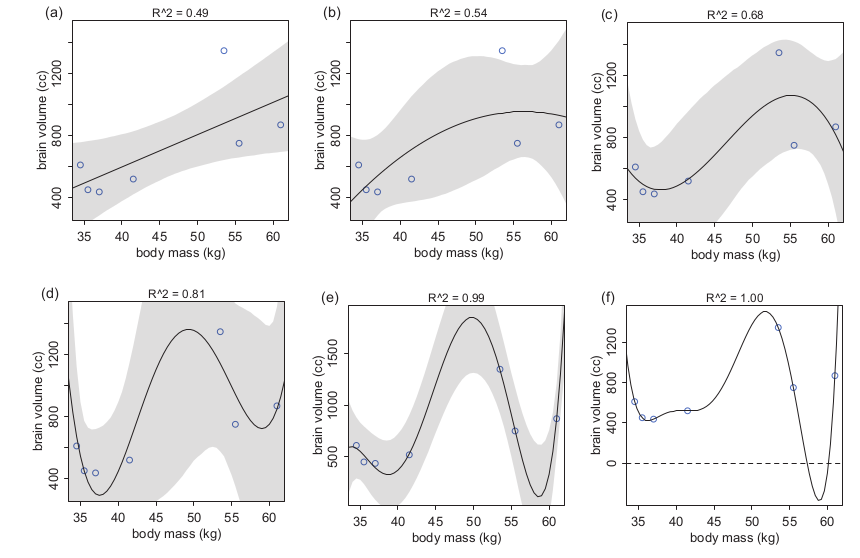
\includegraphics[scale=0.41]{pics/polyover.png}
\end{figure}

Polynomial linear models of increasing degree, fit to the hominin data. Each plot shows the predicted mean in black, with 89\% interval of the mean shaded. $R^2$, is displayed above each plot. (a) First-degree polynomial. (b) Second-degree. (c) Third-degree. (d) Fourth-degree. (e) Fifth-degree. (f) Sixth-degree. Source: \cite{mcelreath2020statistical}. 

} 
\end{frame}




\begin{frame}{The problem with parameters}
\scriptsize{

\begin{itemize}

\item We can see from looking at the paths of the predicted means that the higher-degree polynomials are increasingly absurd. 

\item For example panel (f) shows the most complex model, reg.ev.6.

\item The fit is perfect, but the model is ridiculous. 

\item Notice that there is a gap in the body mass data, because there are no fossil
hominins with body mass between 55 kg and about 60 kg. 
\item In this region, the predicted mean brain size from the high-degree polynomial models has nothing to predict, and so the models pay no price for swinging around wildly in this interval.
\item The swing is so extreme that at around 58 kg, the model predicts a negative brain size!

\item The model pays no price (yet) for this absurdity, because there are no cases in the data with body mass near 58 kg.

\end{itemize}


} 
\end{frame}



\begin{frame}{The problem with parameters}
\scriptsize{

\begin{itemize}

\item Why does the sixth-degree polynomial fit perfectly? 
\item Because it has enough parameters to assign one to each point of data.

\item The model's equation for the mean has 7 parameters:

\begin{displaymath}
 y_i=\beta_{0}+\beta_{1}x_i +\beta_{2}x_i^2 +\beta_{3}x_i^3 +\beta_{4}x_i^4 ++\beta_{5}x_i^5+\beta_{6}x_i^6+\epsilon_i \quad \forall i
\end{displaymath}
and there are 7 species to predict brain sizes for.

\item So effectively, this model assigns a unique parameter to reiterate each observed brain size.
\item This is a general phenomenon: If you adopt a model family with enough parameters, you can fit the data exactly. 
\item But such a model will make rather absurd predictions for yet-to-be-observed cases.


\end{itemize}


} 
\end{frame}


\begin{frame}{Information theory and model performance}
\scriptsize{

\begin{itemize}
\item Blabla
\end{itemize}


} 
\end{frame}


\begin{frame}{Regularization}
\scriptsize{

\begin{itemize}
\item Blabla
\end{itemize}


} 
\end{frame}

\begin{frame}{Information criteria}
\scriptsize{

\begin{itemize}
\item Blabla
\end{itemize}


} 
\end{frame}


\begin{frame}{Using information criteria}
\scriptsize{

\begin{itemize}
\item Blabla
\end{itemize}


} 
\end{frame}




\begin{frame}{Conclusions}
\scriptsize{

\begin{itemize}
\item Blabla
\end{itemize}


} 
\end{frame}


%%%%%%%%%%%%%%%%%%%%%%%%%%%
\begin{frame}[allowframebreaks]\scriptsize
\frametitle{References}
\bibliography{bio}
\bibliographystyle{apalike}
%\bibliographystyle{flexbib}
\end{frame}  









%%%%%%%%%%%%%%%%%%%%%%%%%%%

\end{document}
